% !TEX root = ../termpaper.tex
% @author Leonhard Lüdeke
%
\section{Anhang}
\label{Anhang}

%\label{mas_arch}
%\input{chapters/MAS_architektur_01.pdf}


\begin{figure}
	\centering
	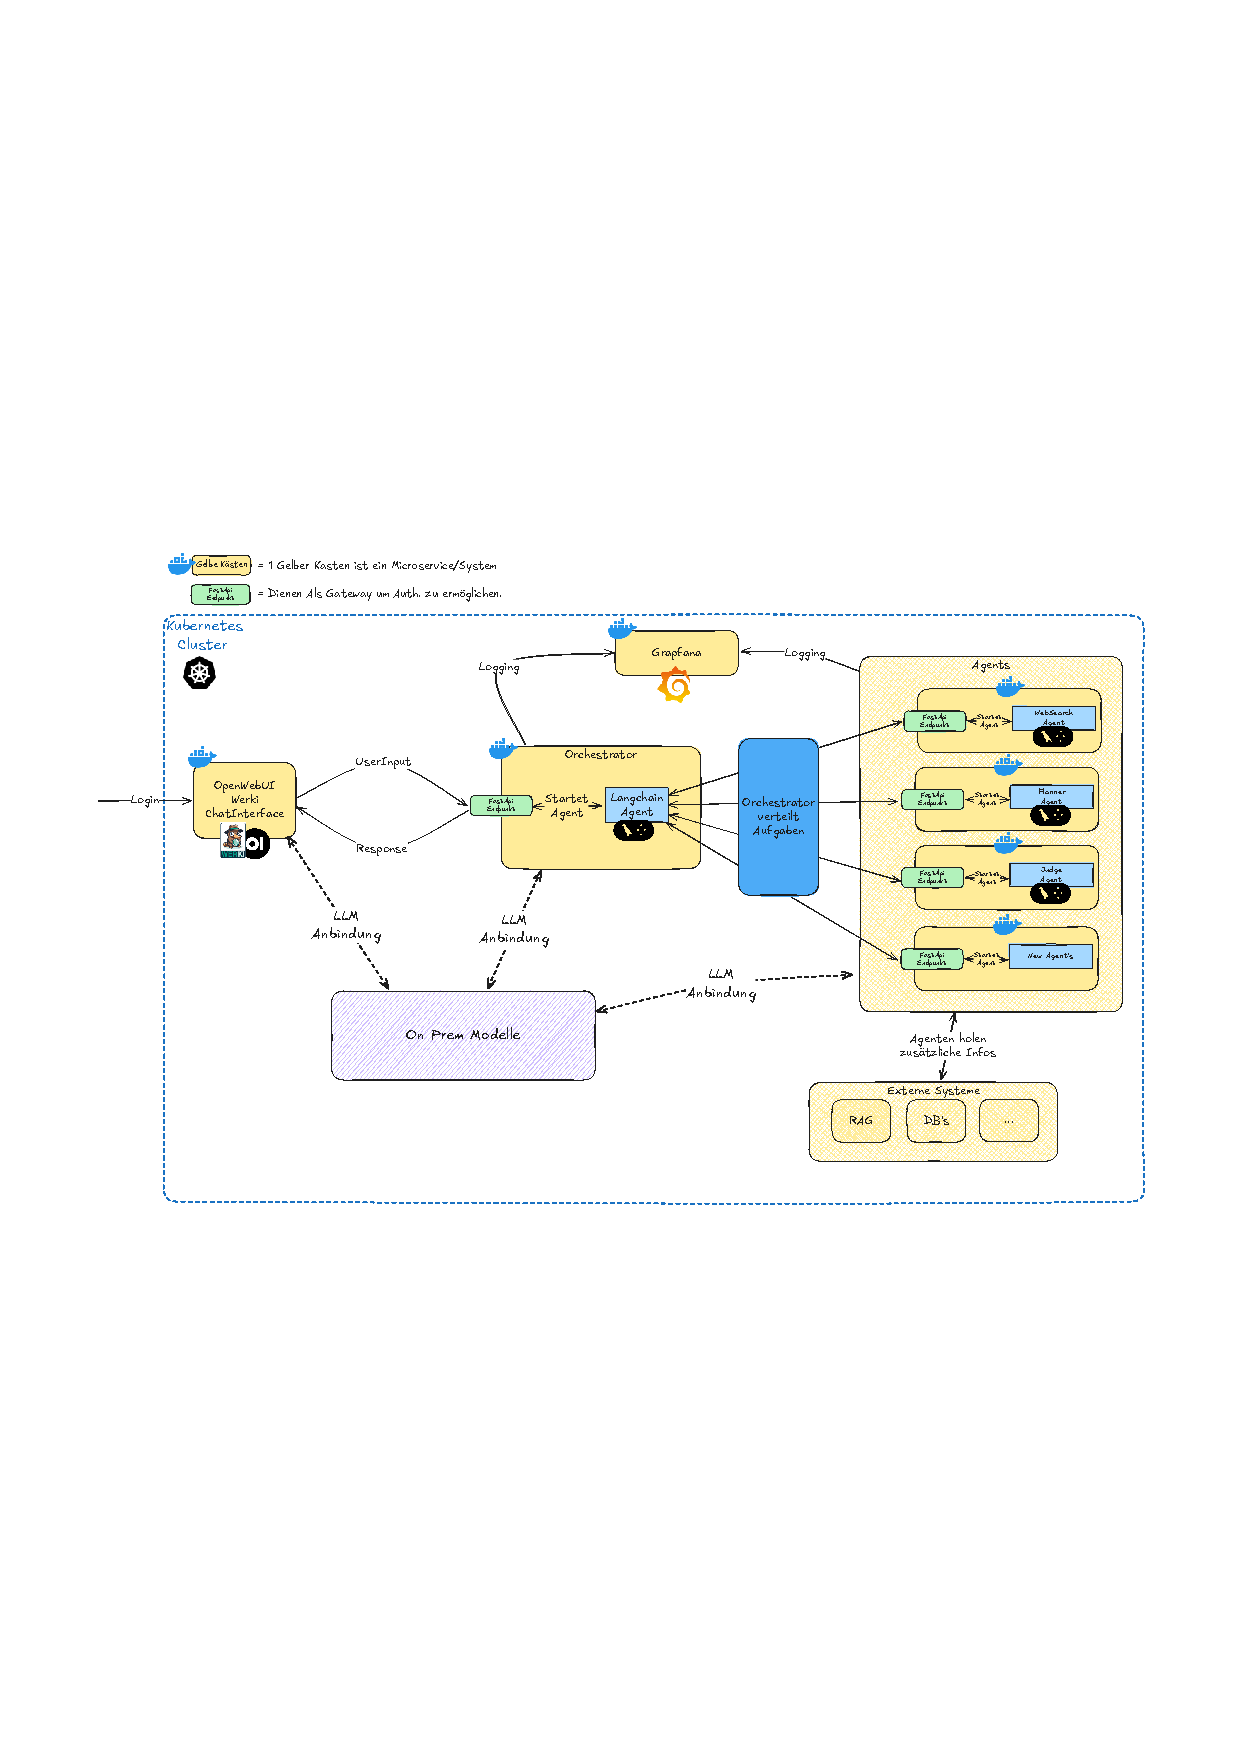
\includegraphics[width=1.0\linewidth]{chapters/MAS Architektur 01.pdf}
	\caption{}
	\label{fig:mas_arch}
\end{figure}

\paragraph{Anwendungsklasse}
\label{Anwendungfälle}

Die Anwendungsfallklasse umfasst komplexe, informations- und dokumentenzentrierte Unternehmensaufgaben, bei denen mehrere spezialisierte LLM-basierte Agenten Informationen aus heterogenen internen und externen Quellen beschaffen, analysieren, zusammenführen und bewerten, um ein nachvollziehbares Arbeitsergebnis zur menschlichen Prüfung oder Entscheidung vorzubereiten.

\subparagraph{Mögliche formulierungen für Anwendungsfälle}

- Assistierte Bearbeitung komplexer wissensintensiver Unternehmensaufgaben
- Agentengestützte Recherche, Analyse und Synthese heterogener Informationen
- Teilstrukturierte, wissensintensive Unternehmensprozesse mit dynamischer Aufgabenzerlegung

\newpage